\section{Multichannel Cross-Layer Routing Protocol}
\label{sec:multichannel}

Multichannel Cross-Layer Routing Protocol (MCRP) concentrates on finding channels for nodes that are free from or have low interference. It allows the allocation of these channels in a way likely to minimise the chances of nodes which are physically near to communicate on the same channel and hence, reduce cross interference between different pairs of nodes.

\subsection{Overview}

The design of the multichannel protocol is based on several crucial observations:
\begin{itemize}
\item Channel assignment - Sensors have limited memory and battery capabilities. In order to maximise the sensors lifetime, a centralised LPBR that has larger memory and fully powered is used for decision making. LPBR has a complete knowledge of the topology which enables it to make good channel assignment decisions based on a two-hop colouring protocol.

\item Interference - External interference cannot be predicted, thus channels cannot be allocated beforehand as it varies over time and locations. It is impossible to determine a single channel that is free from interference at any location. Our protocol checks the channel condition each time before deciding on a channel change to reduce interference and maximise throughput.
%Please consider the following notes on the design:
%- What if the current channel that you are using to communicate channel-switch decision is  too bad that you could not get the message through?
%- Channel conditions change rapidly with time. What about the communication time from the central coordinator to the node?

\item Frequency diversity - Multichannel increases the robustness of the network towards interference. However, applying multichannel to the existing RPL may hinder neighbour detection and RPL processes to maintain the network topology as it does not switch to the correct channel. We overcome this problem by enabling both broadcast on a default channel, and unicast, in neighbour detection and RPL control messages. 

\item RPL - In multichannel, sending a broadcast on every channels would waste the bandwidth. RPL messages are instead sent through unicast when the neighbours are known and broadcast in the default Contiki channel 26 in order to reduce unnecessary transmitting in broadcast. By sending a broadcast on only one channel on which the new neighbours are going to start, the nodes can be discovered and the channel change processes can be performed. 

\item Topology - The topology could change according to the routing metric the way the usual RPL would work. The nodes can still change the parents as usual as all neighbours know each other new channels. The neighbours that are not part of the route do not probe the parent when making the channel decision. However, the neighbours are informed of any channel changes.

\end{itemize}

Our cross-layer multi-channel protocol focuses on the network and application layer of the protocol. This allows channel assignment decisions to be made thoroughly without being limited by the low layer complexity. The channel assignment processes take place only after the topology tree has been formed by RPL and stabilised. The system has two parts: a central algorithm which can be collocated with the LPBR and selects which channel each node should listen on; and a protocol which allows the network to communicate the channel change decision, probe the new channel and either communicate the success of the change or fall back to the previous channel. 

\subsection{Channel Selection Strategy}

One main advantage of the system we propose is it is general and any algorithm can be used at the LPBR to assign channels. In this paper we use a two-hop colouring protocol to select a channel to be assigned to a node. Channels are chosen in a way that ensures no nodes within two hops of each other on the network are listening on the same channel.
This allows fair load balancing on the channels and reduces channel interference that could occur when two nearby nodes transmit together on the same channel. The nodes used in this paper have a transmission range of approximately 20-30 metres indoors and 75-100 metres outdoors \cite{telosb-datasheet}. It could be the case, therefore, that many nodes in a sensor network are in the transmission range of each other and potentially interfered with.
 
All nodes are initialised to channel 26 by default in Contiki since it often has fewer interference problems with Wi-Fi and other sources. The studies in \cite{chrysso, micmac, watteyne} use whitelisted channels in their experiments and have channel 26 in common. The usual RPL set up mechanism is used to exchange control messages that are required to form an optimised topology before channel assignments can take place. The nodes will only be on the same channel once during the initial setup.  
	
In the two-hop colouring protocol, the LPBR chooses a node to which it will assign a channel to listen on. The selection is random (from channels 11 to 26) based on the full range available \cite{ieee802.15.4}. The protocol checks neighbours and neighbours of neighbours to see if any of those are listening on this channel already. If any are, a new channel is picked from the remaining list of available channels. If the LPBR has knowledge of existing bad channels then those channels can be blacklisted.  Knowledge of channel interference which is gained by probing can be used to decide that a channel should not be used. If a channel is found then the channel switching protocol is triggered. If no channel can be found meeting these conditions, the current channel is kept.  

The node selection algorithm must only attempt one channel change at a time to ensure probing is done on the correct new channel and for the node to finalise the channel to be used before another node tries to attempt a channel change.
The protocol ensures that the channel change attempt will always result in a message returned to the LPBR either confirming the new channel or announcing a reversion to the old channel. Until one or other of these happens, no new channel change will be made to ensure that the neighbours are transmitting on the correct channel.

\subsection{Channel Switching}
\label{sec:channelswitch}

\begin{figure}
\centering
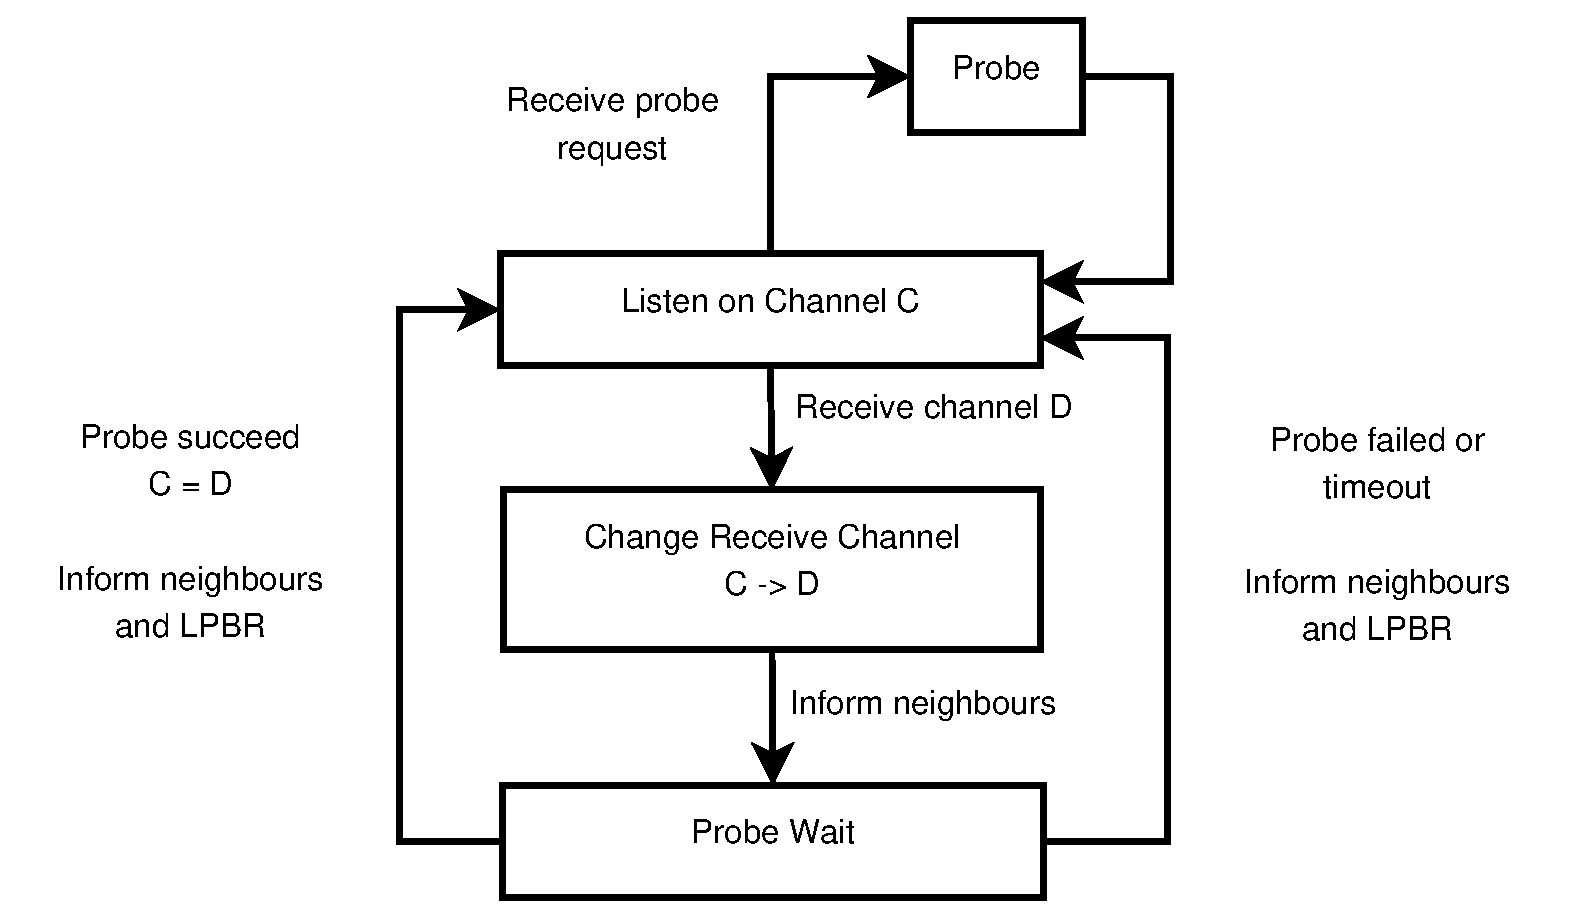
\includegraphics[width=3.5in]{Diagram1.eps}
\caption{Channel switching processes}
\label{fig_sim}
\end{figure}

Figure \ref{fig_sim} shows the state machine for the channel switching protocol.
As explained in the previous section, a choice of a new channel by the channel selection protocol causes a change channel message to be sent to the appropriate node. 
On receiving a channel change message a node $N$ stores its current channel $C$ and communicates to all its neighbours the new channel $D$ it wishes to change to.  Those neighbours will update their neighbour tables to ensure that they now send to node $N$ on channel $D$.  The node $N$ now begins the channel quality checking process (see section \ref{sec:channelquality}) with each neighbour in turn by sending them a probe request.  If this process fails for any neighbour then the node reverts to channel $C$.  Node $N$ informs its neighbours of this reversion to channel $C$ and informs the LPBR of the channel checking results and its reversion to listening on channel $C$. If all channel quality checks succeed, the node $N$ will listens on channel $D$. It is important to emphasise that the network remains fully functional and connected at all stages of this protocol (however, the channel checking process uses probe packets that might interfere with other transmissions temporarily).

\subsection{Channel Quality Checking}
\label{sec:channelquality}

In describing the channel quality checking process it is worth emphasising the RPL distinction between neighbours and tree neighbours. In RPL, node neighbours are all nodes that a given node knows it could transmit to. Tree neighbours are the nodes that a node does transmit to through the topology formed by the RPL protocol.

The channel quality checking is invoked each time a node changes channel after receiving a message from the LPBR. A node $N$ changing to channel $D$ informs all neighbours in turn, of the new channel $D$ it will be listening on as described in the previous section. It then enters the Probe Wait state and begins channel quality checking with each tree neighbour in turn.  

In the Probe Wait state node $N$ sends a Probe message to each neighbour in turn. That neighbour will respond to the message by sending eight packets to $N$ on the new channel $D$. If this process times out (because of some communication failure) or the number of probe packets received is below a threshold (currently set to 16) then node $N$ immediately exits Probe Wait and reverts to channel $C$ its previous channel. 

The buffer can accommodate eight packets at a time. As the packets might not be sent immediately due to wakes up and collisions, sending more packets would have the risk of being dropped. Increasing the buffer size is not ideal as the sensor has limited memory capability. However, as the numbers of probing packets are small, the estimate value might not be accurate as the representation of the channel condition. The condition of the channel is further investigated through the number of retransmissions and packet collisions of the probing packets. 

The threshold is set to be 16 (including retransmissions and collisions) to ensure that moderate interference channels are avoided. Mild interference channels usually fall below the threshold. If the threshold is not met, none of the node would change the channel as the node would be better off with its current channel. 

All neighbours are informed of the change back to channel $C$ and the LPBR is informed of the quality check failure with a summary of all probes received.
If, on the other hand, all channel quality checks succeed the change to channel $D$ becomes permanent for node $N$ and it informs the LPBR of the results of the probing (numbers of packets received) and the channel change.

Probing is an important part in making the channel change decision. It gives a quick overview of the channel condition based on the number of probing messages received. It is worth noting that probing is only done between the node and the tree neighbours. Neighbours that are not tree neighbours will not use the node as a route during their transmission thus, there is no need for probing to take place with those neighbours. However, the neighbours still need to know the channel value as RPL control messages are sent to neighbours directly without using the routes.
